\section{Results}
\label{results}
%From ILO:
%"Plan and carry out a small-scale investigation of an algorithmic research problem. This investigation could be theoretical, experimental, or both."
This sections describes the results reached in the project. The goal in this section is threefold. Firstly to verify the results achieved in \cite{wagner17}. Secondly to explore the performance of \qs{} on new datasets. These datasets will have different properties than the datasets tested in \cite{wagner17}. Lastly to discover the performance of \qsr{} and compare this to the performance of \qs{}. 
\\
\\
The expirements are based on two datasets from the paper as well as two new datasets.\footnote{From \cite{wagner17} we use the datasets \sift{} and \mnist{}. Explicitly in this paper we have included \clust{} and \gist{}} For each dataset the results of \qs{} is verified and compared to the baseline implementation \gr{} and to \qsr{}. 
\\
\\
The results of these tests are illustrated as line charts. The charts visualizes the performance of the algorithms for each dataset measured in terms of \textit{accuracy pr bit of precision} and \textit{distortion pr bit of precision}. 
\\
\\
Similarly as in \cite{wagner17} the \qs{} implementations has been parameterized with \textit{L} ranging from 2 till 10 and $\Lambda$ ranging from \textit{L$_{min}$-1} to \textit{L$_{max}$-1}.\footnote{Their experiments range from \textit{L} ranging from 2 till 20 and $\Lambda$ 1 till 19. However the computation time for trees with a depth $>$ 14 is immense.} 
%\subsection{Practical improvements}
%Instead of randomly shifted ( works well for arbitrary, but maybe we know our data )
%On specific datasets:
%- Scale on spread out datasets, to avoid one point in each quad leaf
%- Zoom in on narrow / close datasets
\\
\\
The charts presented first displays results from the datasets \mnist{} and \sift{}. These results are key in verifying the results presented in \cite{wagner17}. Following this are the charts displaying results from \clust{} and \gist{}, as these disclose new information about the overall performance of \qs{}. Two graphs exists for each dataset displaying \textit{accuracy} and \textit{distortion} respectively.
\begin{figure}[h]
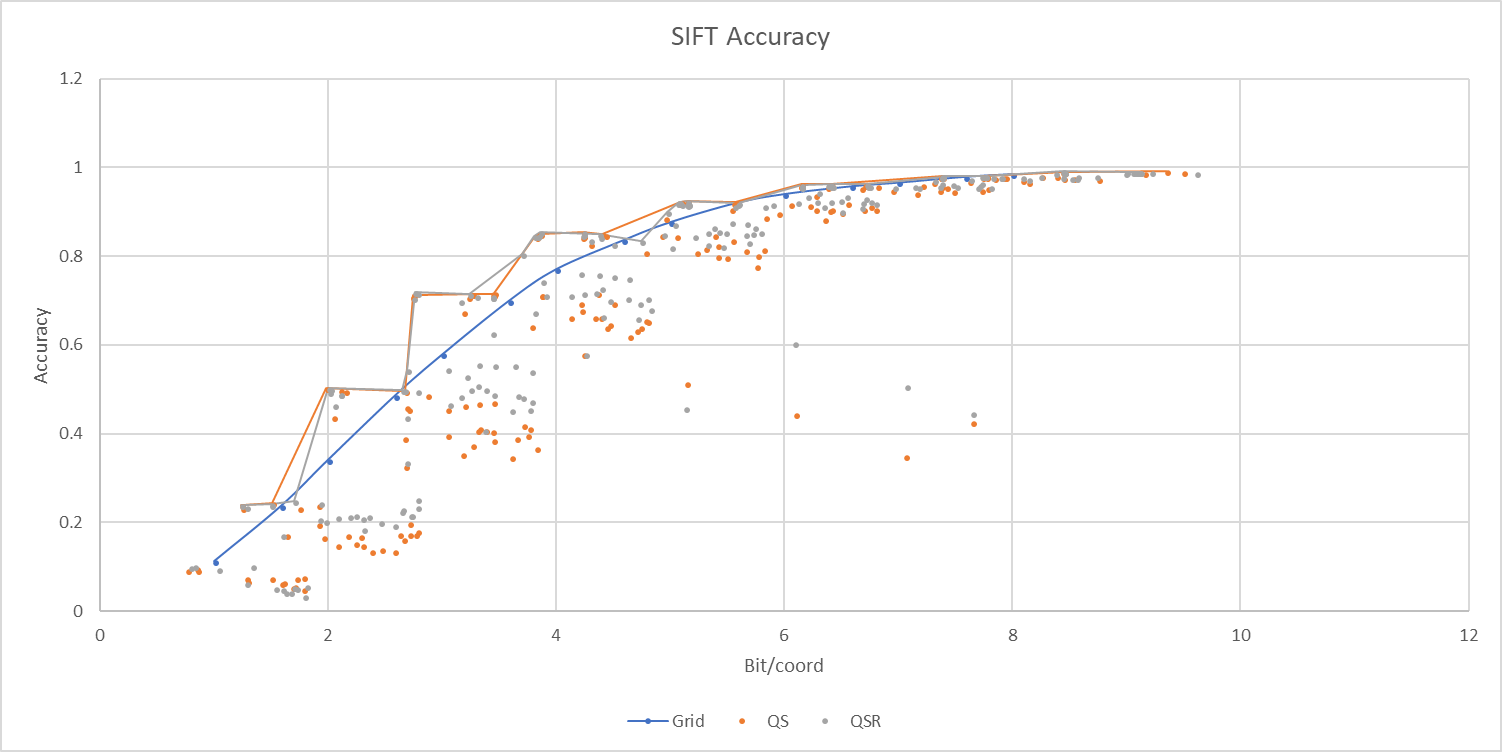
\includegraphics[width=0.5\textwidth]{figures/graphs/sift_accuracy}
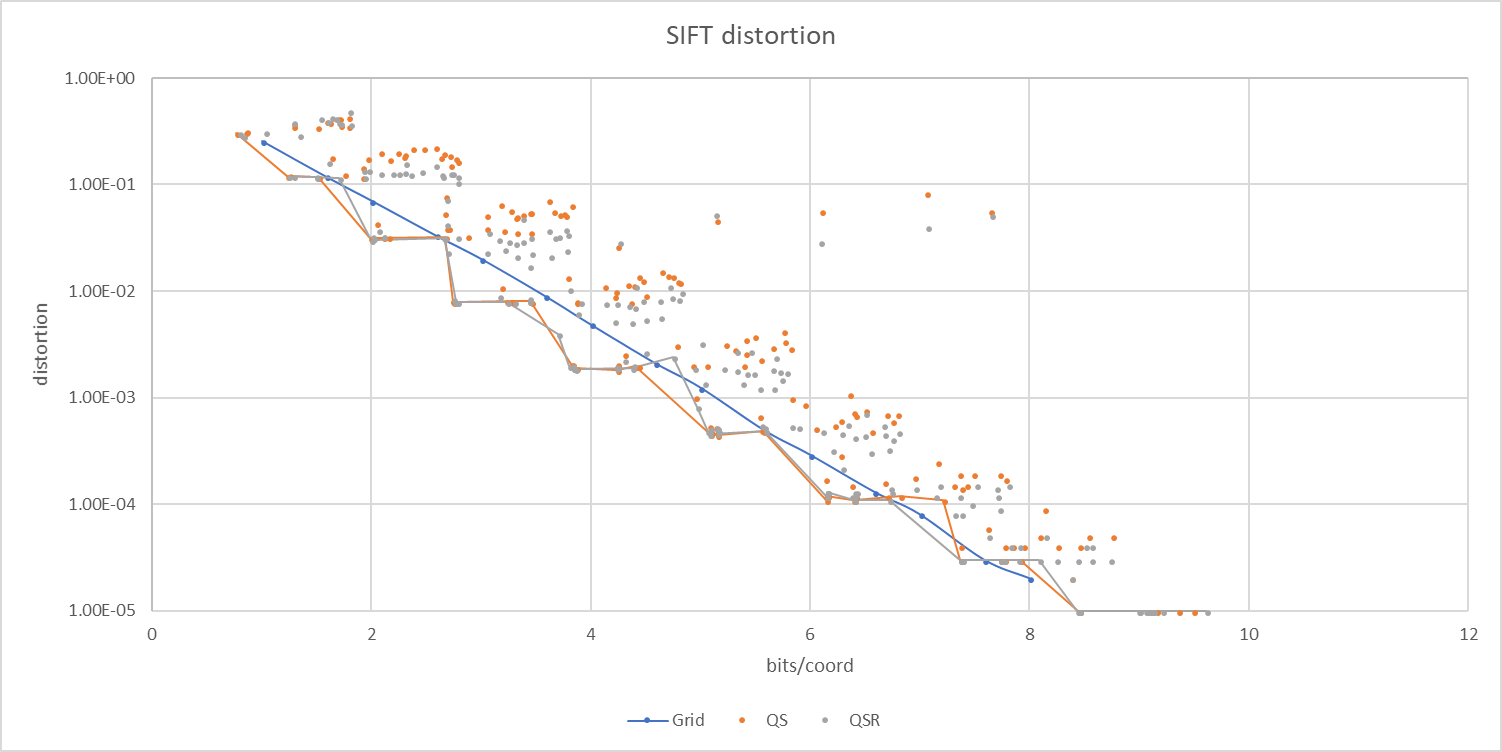
\includegraphics[width=0.5\textwidth]{figures/graphs/sift_distortion}
\caption{Accuracy and distortion from \sift{}}
\label{fig:graph sift}
\end{figure}
\clearpage{}
The results from Figure \ref{fig:graph sift} verifies the original results of \qs{}, and establishes that it still outperforms the baseline method. Interestingly the \qsr{} implementation has fewer bad cases, which could indicate that on the..............

\begin{figure}[h]
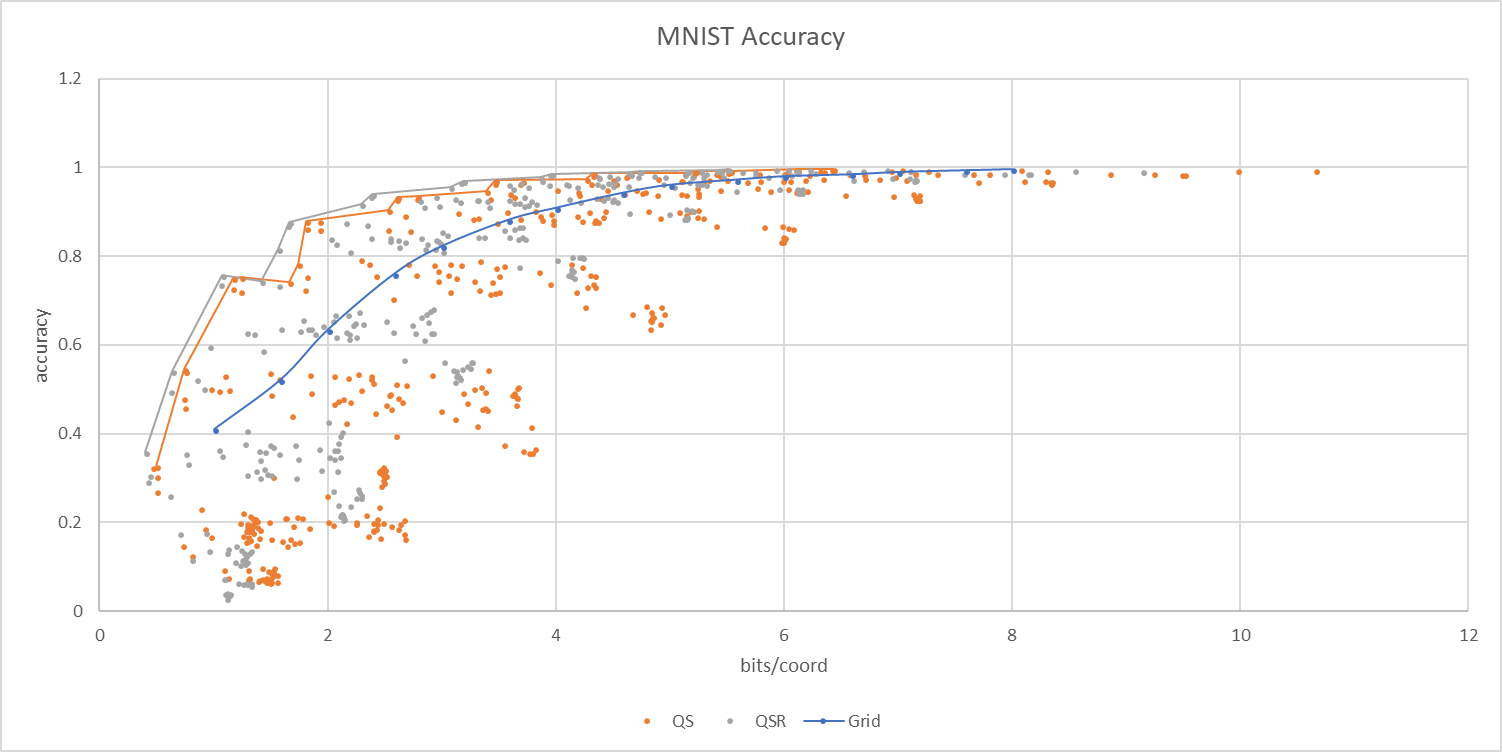
\includegraphics[width=0.5\textwidth]{figures/graphs/mnist_accuracy}
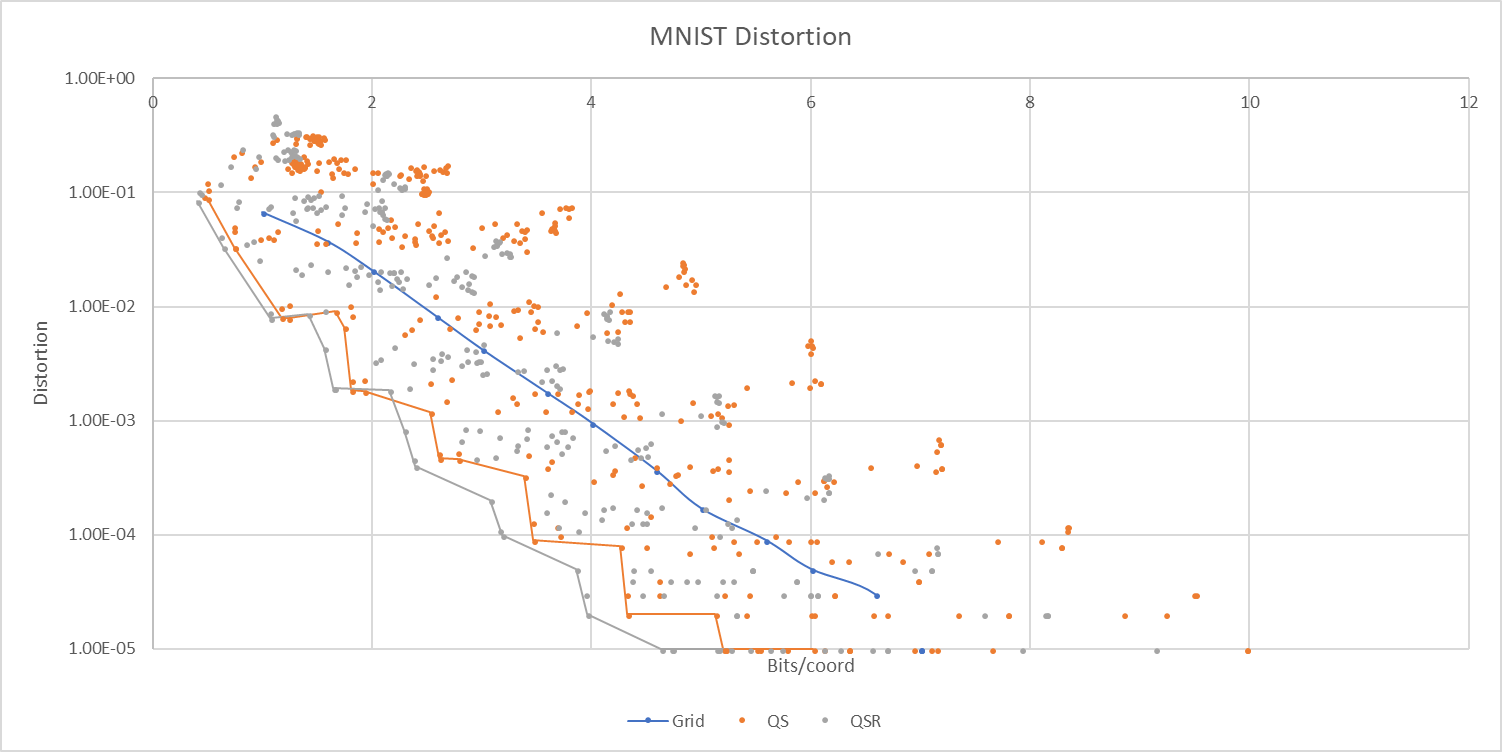
\includegraphics[width=0.5\textwidth]{figures/graphs/mnist_distortion}
\caption{Accuracy and distortion from \mnist{}}
\label{fig:graph mnist}
\end{figure}
Here we now describe our amazing results from mnist. Probably we will be rich from these results. If not, Erlich Bachmann will be very disappointed (remember, that Bakke still lives in his incubator). 

\begin{figure}[h]
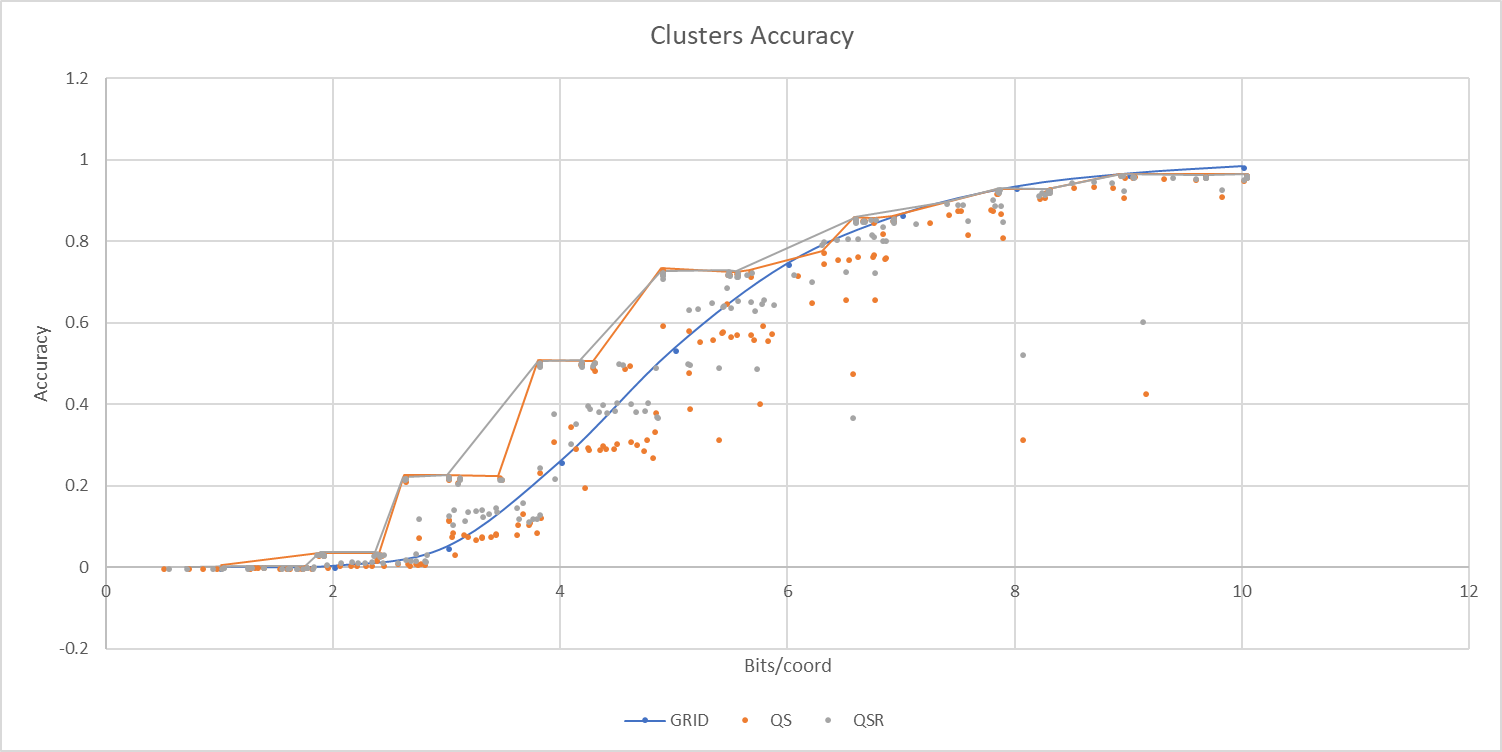
\includegraphics[width=0.5\textwidth]{figures/graphs/clusters_accuracy}
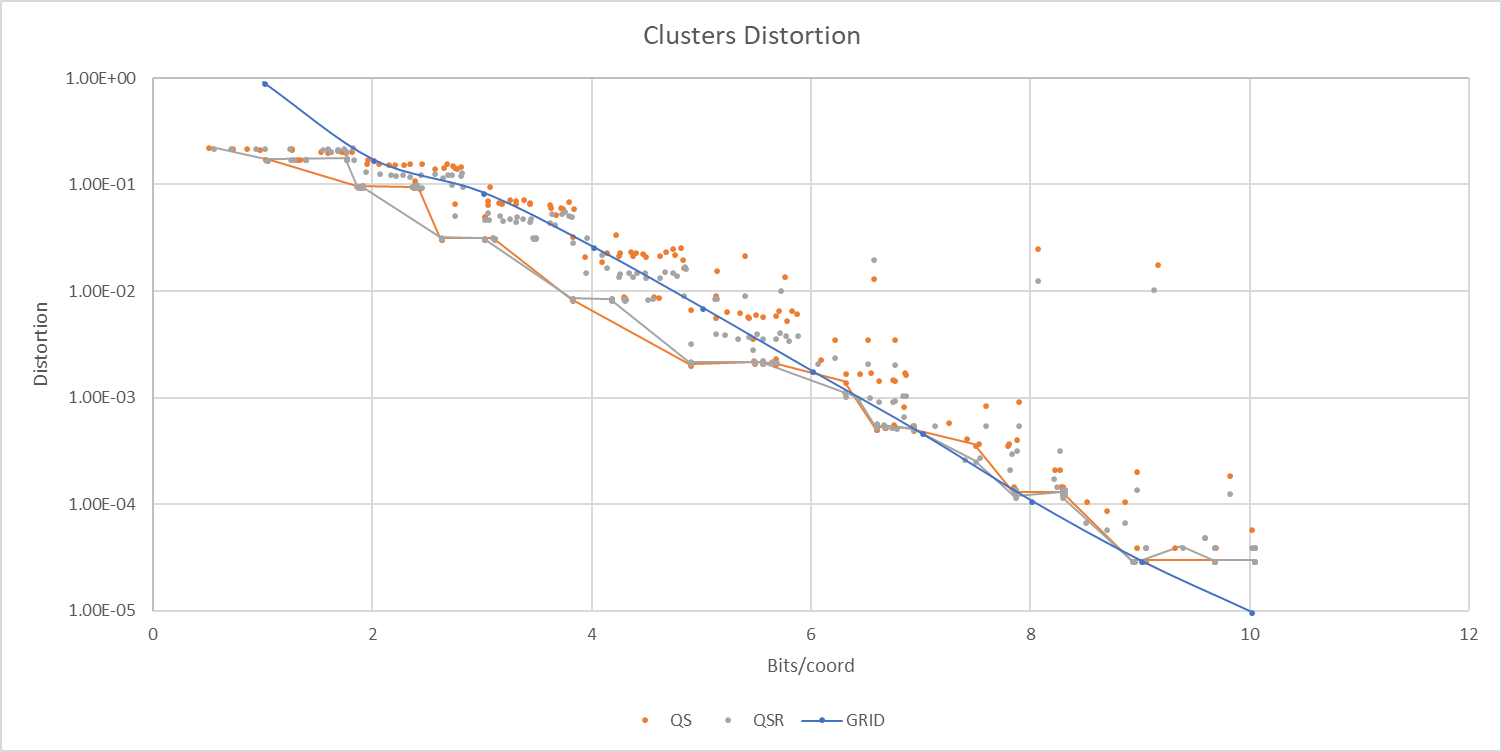
\includegraphics[width=0.5\textwidth]{figures/graphs/clusters_distortion}
\caption{Accuracy and distortion from \clust{}}
\label{fig:graph clust}
\end{figure}
Here we now describe our amazing results from clust. With our incredible weismann score on 10.9, beating Richards score by a factor 4, we now should be able to build a new internet. However, if we are unlucky, Ying Yang will beat us to it....
\clearpage{}

\begin{figure}[h]
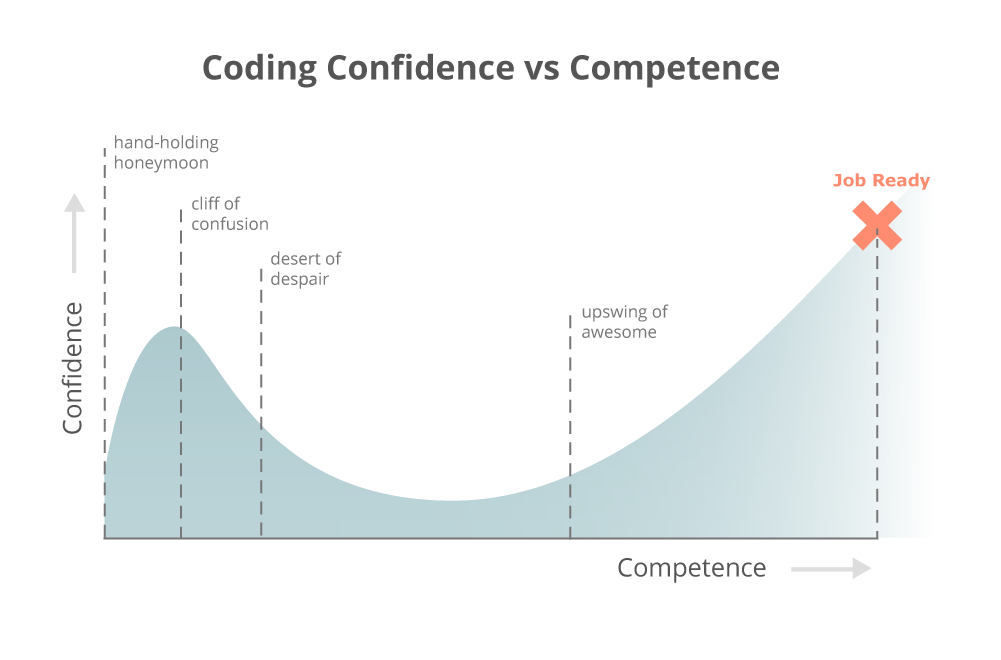
\includegraphics[width=0.5\textwidth]{figures/coding_graph}
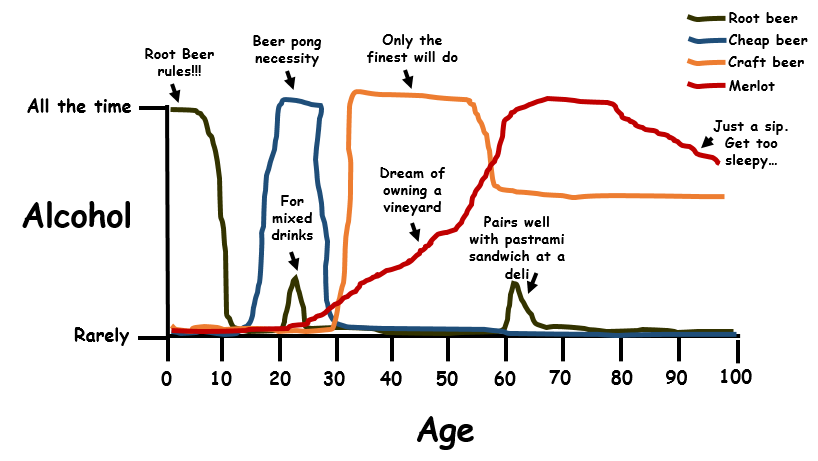
\includegraphics[width=0.5\textwidth]{figures/alcohol_graph}
\caption{Accuracy and distortion from \gist{}}
\label{fig:graph gist}
\end{figure}
Gist is the last dataset to demonstrate our extreme improvemnts. I am quite sure that we will impress Johan and Sam. And Erlich Bachmann (all heil). GG maybe this will not appear at all since the tests take a day to run each...

